\subsection{Descripci\'on del problema}

En este ejercicio se nos pide escribir un algoritmo que resuelva una especie de rompecabezas dado por un tablero de $n \times m$ casillas y $n \times m$ fichas.
Cada pieza (cuadrada) tiene un color en cada uno de sus lados, no necesariamente colores distintos en cada uno. Por ejemplo: 

\begin{figure}[h]
\begin{center}
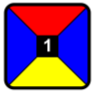
\includegraphics[scale=0.4]{./img/ej3_fichas.png}
\caption{Ejemplo de ficha}
\end{center}
\end{figure}

Ahora, para poder poner una pieza en el tablero debemos asegurarnos de que los colores de los lados coincidan con los de las fichas adyacentes (en caso de que haya una ficha lindante). Un ejemplo de las posicionamiento correcto e incorrecto ser\'ia:\\

\begin{figure}[h]
\begin{center}
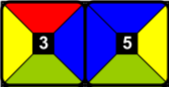
\includegraphics[scale=0.4]{./img/ej3_fichas_coinciden.png}
\caption{Ejemplo posicionamiento correcto}
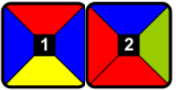
\includegraphics[scale=0.4]{./img/ej3_fichas_ncoinciden.png}
\caption{Ejemplo posicionamiento incorrecto}
\end{center}
\end{figure}

 M\'as all\'a de esta restricci\'on, cualquier pieza puede colocarse en cualquier casillero.\\
El modo resolutivo del rompecabezas no necesariamente debe ser total, ya que el conjunto de piezas dado podria no tener un ordenamiento tal que pueda llenar completamente el tablero, por lo tanto, la soluci\'on al problema debe ser lo m\'as \'optima posible, aquella en la que mayor cantidad de piezas permita ingresar en el tablero dadas las restricciones anteriores.
Por ejemplo el siguiente gr\'afico muestra una soluci\'on \'optima, dado un conjunto de piezas que no permiten llenar por completo el tablero.

/*Imagen editada del enunciado*/

Para la resoluci\'on del rompecabezas, no se pueden girar las piezas por más que esto permita llegar a una mejor soluci\'on. La postura de las piezas es la dada.

\subsection{Resoluci\'on}

Para resolver este problema se nos pidi\'o utilizar la t\'ecnica algor\'itmica de backtracking. Por lo tanto utilizando esta misma comenzamos situados en el primer casillero (superior izquierdo) movi\'endonos de izquierda a derecha y de arriba hacia abajo en el tablero. La idea del algoritmo de backtracking es ir probando todas las combinaciones posibles de cada pieza (incluida la pieza en blanco o vac\'ia) en cada casillero del tablero comparando todos los tableros obtenidos y qued\'andose con el mejor de todos estos, el m\'as \'optimo, en el que mayor cantidad de piezas no vac\'ias se lograron poner.

/*PseudoCodigo del recorrido del tablero*/

Con este prop\'osito y para optimizar el algoritmo creamos un tablero de referencia, en el cual iremos guardando el tablero v\'alido, con la mejor combinaci\'on, por ende con la mayor cantidad de piezas (no vac\'ias), obtenido hasta el momento.

La idea de el tablero de referencia surge a la hora de pensar posibles podas para el \'arbol formado por la recurci\'on del algoritmo de backtranking, ser\'ia innecesario tener que probar absolutamente todas las combinaciones posibles de fichas en casilleros del tablero ya que es obviamente visible que una gran parte de estas no serian o llegar\'ian a ser una soluci\'on \'optima, como puede ser el tablero completamente vac\'io, o el tablero con menos de la mitad de las casillas llenas.

Por lo tanto las podas implementadas son las siguientes:

\begin{itemize}

\item La primer poda consiste en: Una vez que se terminaron de probar las fichas disponibles en cada casillero del tablero, se debe poner una ficha en blanco (o vac\'ia), en este momento comparamos la cantidad de fichas puestas (no vac\'ias) en el tablero de referencia contra la cantidad de fichas puestas (no vac\'ias) en el tablero actual, más los casilleros que todav\'ia no se recorrieron. Si el valor dado por el tablero actual es igual o menor al valor dado por el tablero de referencia, esta rama del backtraking es podada porque aunque se pudieran colocar fichas en todos los casilleros restantes, no se llegar\'ia a una soluci\'on más optima que la ya obtenida (tablero de referencia). Aqu\'i se regresa al nodo anterior del arbol, cambiando la ficha puesta en este y continuando con el algoritmo.

/*Pseudo c\'odigo de la primer poda*/

\item La segunda poda viene de la mano de la primera, esta consiste en: Antes de comenzar el algoritmo resolutivo se llena el tablero de referencia en posiciones intercaladas de manera que no importa que fichas coloquemos, al no haber dos fichas adjuntas, cualquier combinaci\'on de fichas ser\'a v\'alido. De esta forma obtenemos un tablero con la mitad de los casilleros llenos. Ahora cuando comience el algoritmo en el caso que las primeras ramas del \'arbol de backtracking resulten menos \'optimas que el tablero de referencia obtenido, no llegaran a completarse, porque se cortaran como resultado de la primer poda.

/*Pseudo del llenado del tablero*/

\item La tercer poda es la m\'as intuitiva y simple y consiste en: Si alguna rama de la recursi\'on se llega a la soluci\'on m\'as \'optima posible, esto es obtener el tablero lleno completamente con fichas no vac\'ias, se cortan todas las ramas restantes y se termina el algoritmo. De ser posible, si se llega a tener el tablero completo, no tiene sentido seguir buscando otras combinaciones, ya que no se podria llegar a una mejor soluci\'on.

\end{itemize}

\subsection{Demostraci\'on de la resoluci\'on}

\subsection{Complejidad del algoritmo}

\subsection{Codigo fuente}

\subsection{Casos de prueba}

\subsection{Performance}
